% !TEX encoding = UTF-8 Unicode
%!TEX TS-program = xelatex
\chapter{绪论}
\section{液体火箭纵向耦合振动问题的提出}
纵向耦合振动是由于大型液体火箭结构与管路推进系统相互作用而产生的一种不稳定振动\cite{Rubin:1966, Rubin:1970, Rubin:1973}。结合国内外大量历史资料,可以看出自上世纪六十年代初美国的雷神/阿金钠运载器\cite{Leadbetter:1965, Rubin:1966}和法国的EMERAUDE(VE121)\cite{Dordain:1974}运载器开始,许多大型液体火箭运载器在发射升空过程中都经历了较为严重的纵向耦合振动。由于这种振动的形态和“跳跃的弹簧单腿高跷”类似,所以又被研究者们戏称为POGO振动\cite{Rasumoff:1973}(图\ref{POGO-Analog}),其典型的时域历程如图\ref{Typical:POGO}所示。

\begin{figure}[hb]
  \centering
  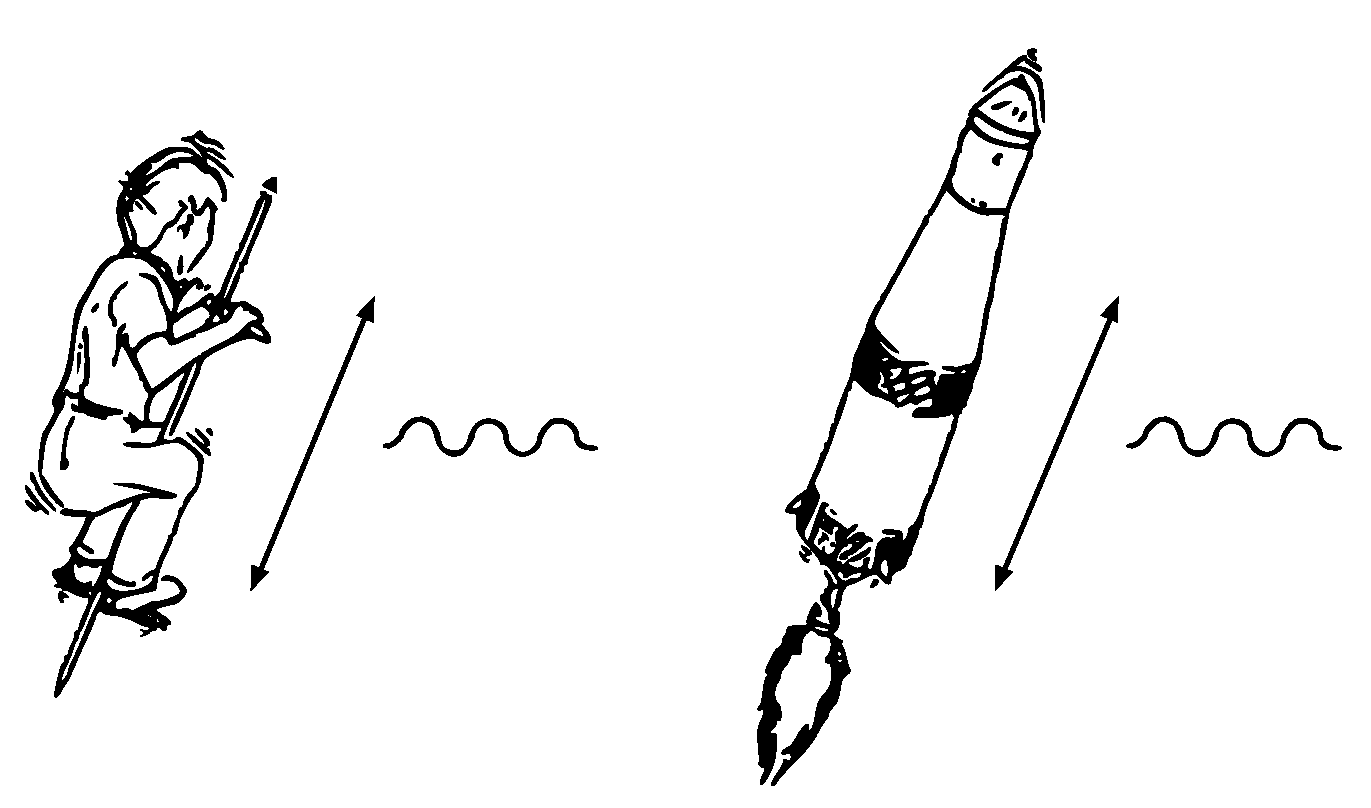
\includegraphics[width=.65\linewidth]{POGO-Analog}
  \caption{POGO比拟示意图}\label{POGO-Analog}
\end{figure}

\begin{figure}[th]
  \centering
  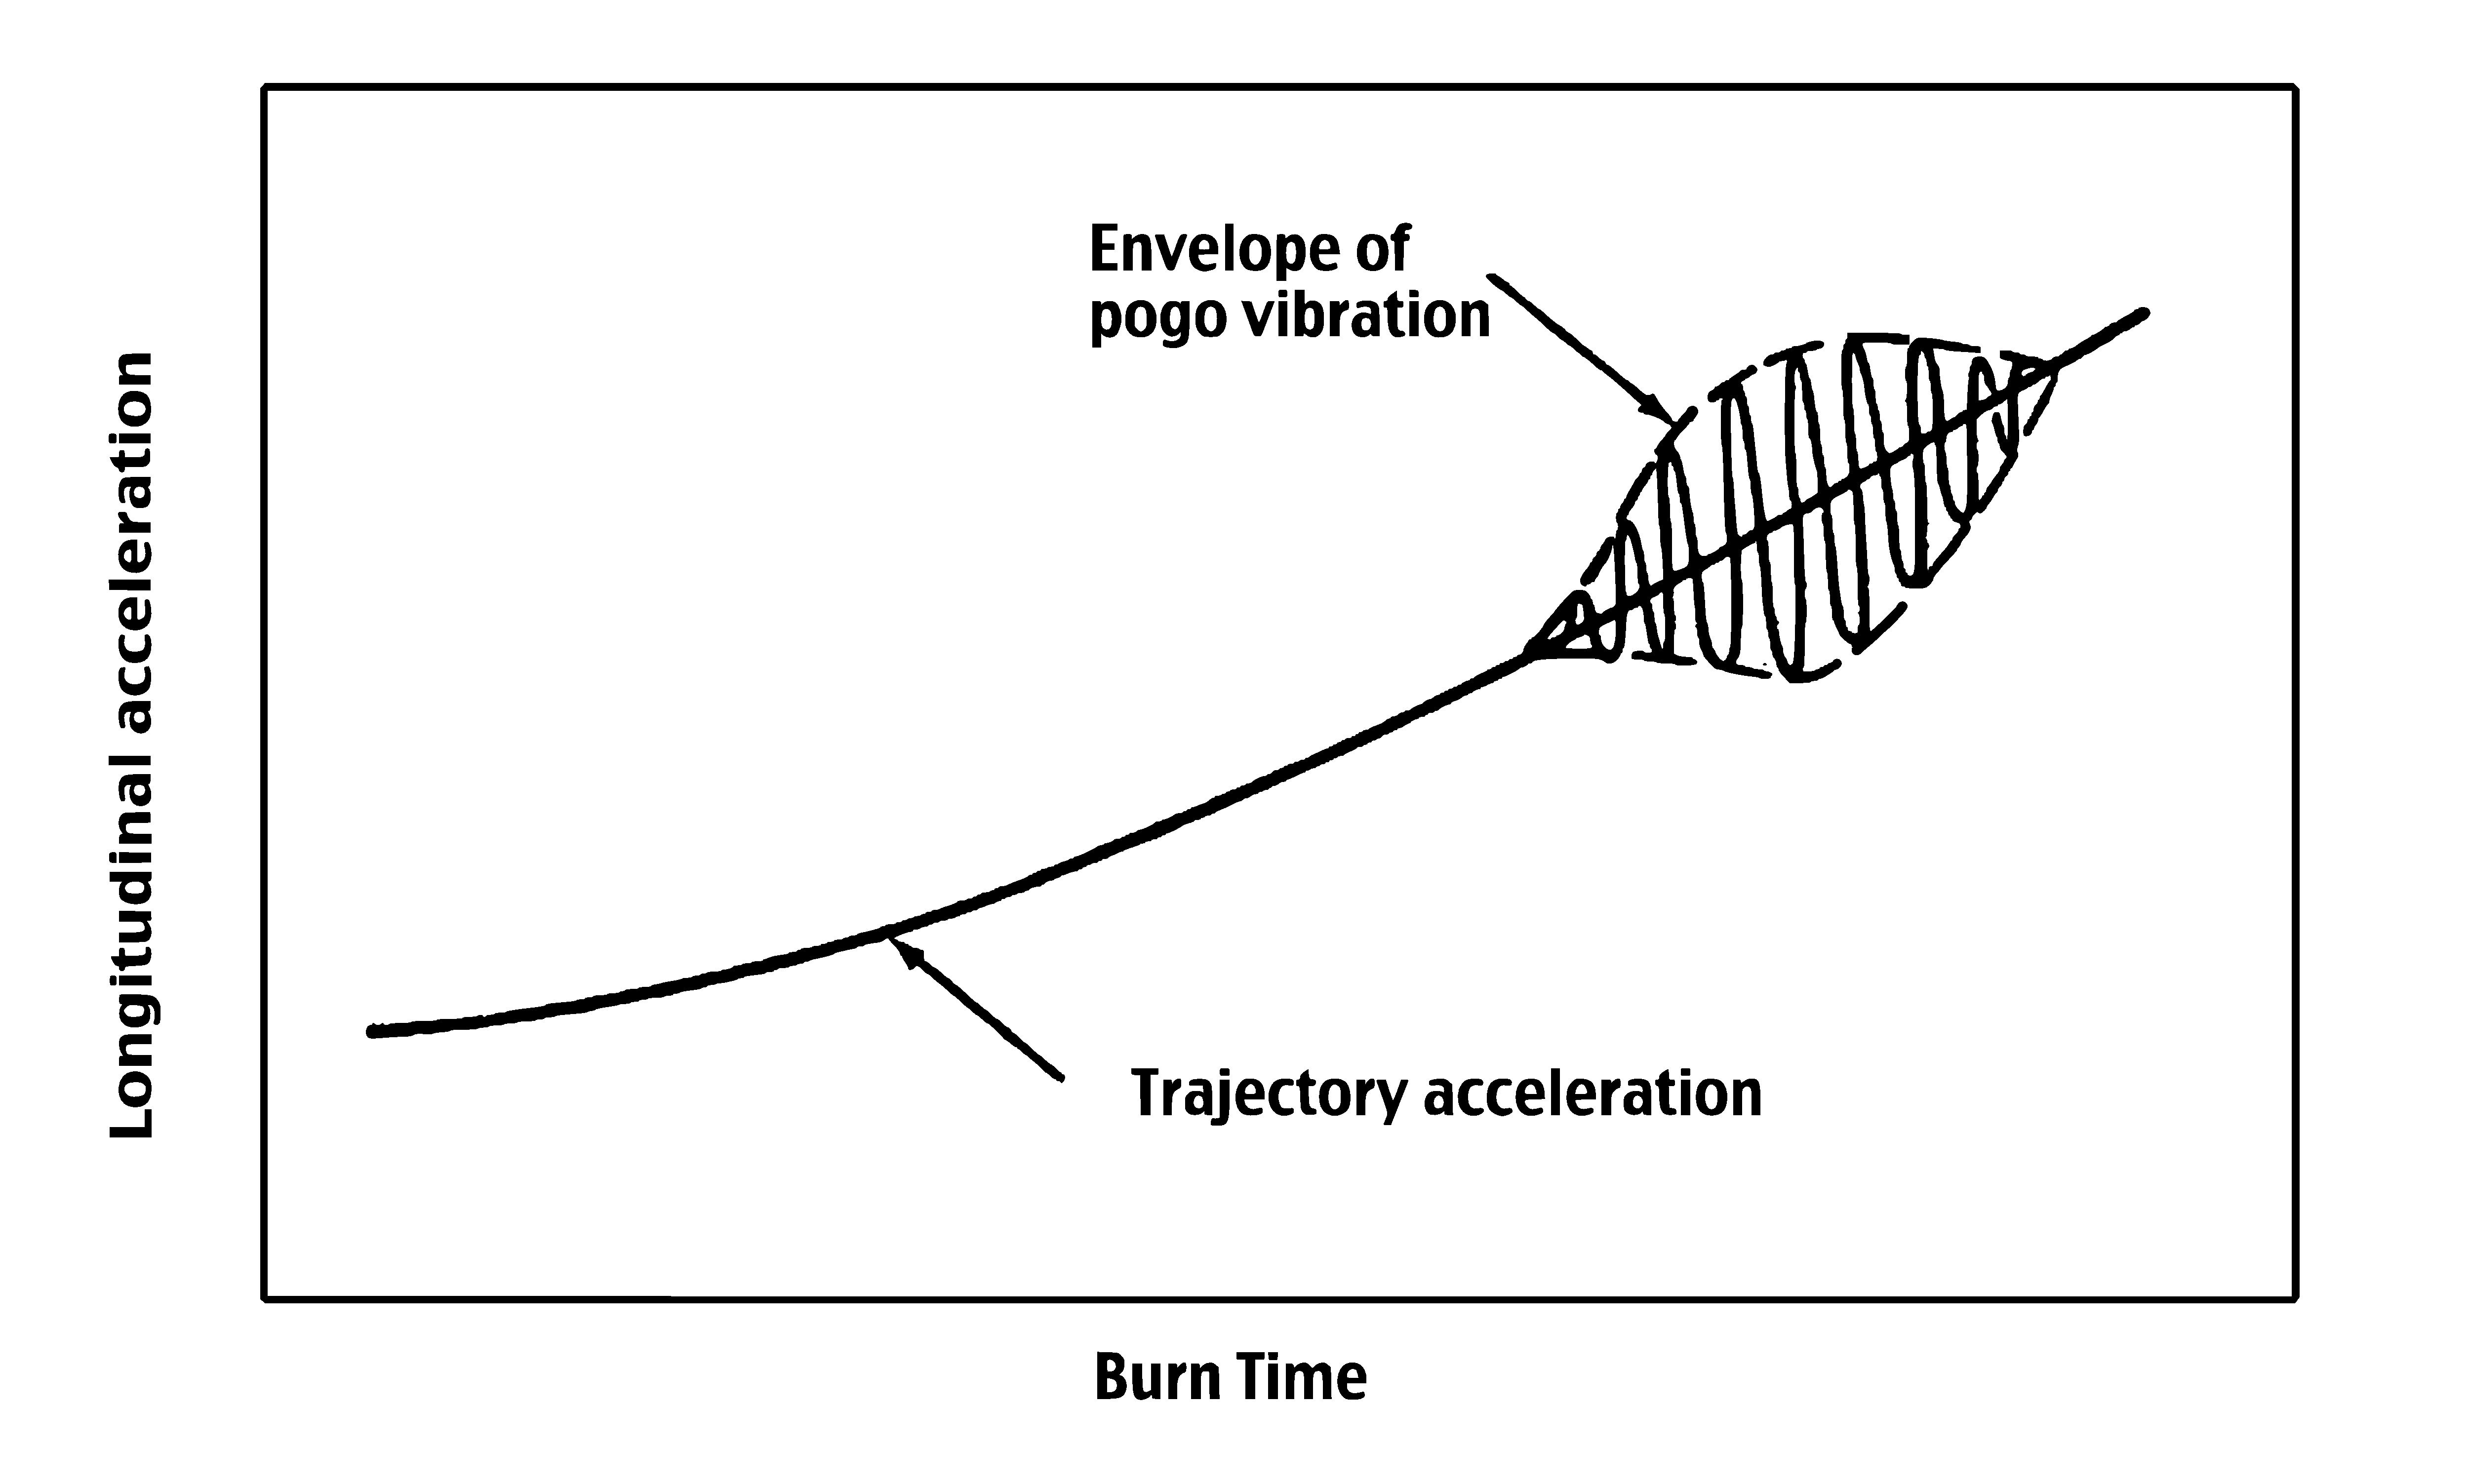
\includegraphics[width=.75\linewidth]{POGO-Typical.pdf}
  \caption{典型纵向耦合振动的时域历程}\label{Typical:POGO}
\end{figure}

纵观现代火箭工程发展史,POGO振动有害于人类航天飞行的典型例证当属美国土星V运载器的一系列发射经历\cite{Hill:1969, Rich:1969, Jarvinen:1970}。土星V运载火箭是美国最大的运载器,是美国国家航空航天局(NASA)在阿波罗计划和天空实验室两项太空计划中使用的多级可抛式液态燃料火箭。事实上,在其总共多达十三次的发射经历中,数次都受到了POGO振动问题的困扰\cite{Larsen:2008}。在1968年土星V编号AS-502次的发射过程中,液体火箭一级推进器(图\ref{SaturnV-Stage1})在工作段105$\sim$140秒内发生了振动频率为5.3Hz,幅值约0.33g的POGO振动。振动导致了五个发动机推力不同步,最终使得飞船登月舱裙部壁板发生开裂。同年十二月发射的土星AS-503,在发动机关机前50秒出现了振动频率为18Hz的POGO振动。事后调查表明,此次主发动机机架与贮箱底部产生的谐振虽然没有传递到火箭壳体,但是已经非常接近简体结构的设计强度极限。在1969年第AS-507次飞行中,液体火箭二级发动机在工作期间出现了四次严格意义上的POGO 振动,所幸最终都被结构系统的非线性效应所遏制。然而,在1970年土星V执行阿波罗13号任务的时候(AS-508),严重的POGO振动导致主发动机机架产生了频率为16Hz,加速度高达68g的失稳现象。由于燃烧室内压力脉动过于剧烈,火箭中部的5号推进器在二级火箭燃烧过程中发生了提前关闭(图\ref{SaturnV-Stage1}),最终导致登月任务被迫放弃,调查发现发动机机架总共被拉长了约7.6厘米。除此之外,宇宙神、大力神和雷神等航空运载器也都在各自发射过程中出现了或多或少的POGO振动\cite{Walker:1964, Wagner:1970, Oppenheim:1993};而法国钻石B火箭更是在其初次发射的五次飞行中都遇到了POGO振动,并且箭体上部分位置的振动量级已然高达足以导致运载器或者卫星结构发生破坏的20$\sim$30g\cite{Dordain:1974}。反观我国的航天事业,在2003年运载火箭长征2F第五次飞行中,遥测数据与宇航员的感受均显示一级助推器飞行末期火箭产生了比较强烈的振动\cite{Ma-Daoyuan:2010, Rong-Kelin:2011}。

\begin{figure}[t]
  \begin{center}
  \begin{minipage}{.47\linewidth}
    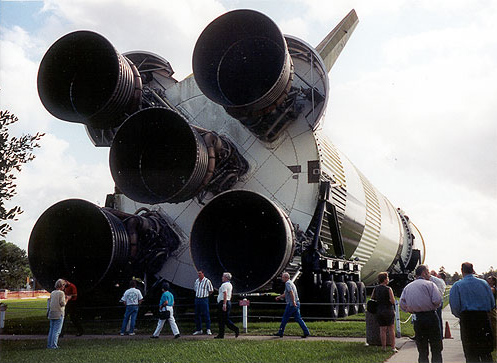
\includegraphics[width=\linewidth]{SaturnV-Stage1.jpg}
    \caption{土星V一级推进器 S-IC}\label{SaturnV-Stage1}
  \end{minipage}
  \begin{minipage}{.47\linewidth}
    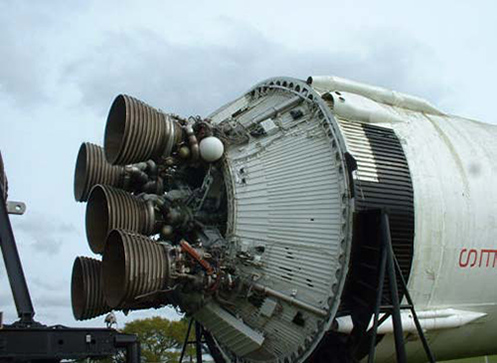
\includegraphics[width=\linewidth]{SaturnV-Stage2.jpg}
    \caption{土星V二级推进器提前关闭}\label{SaturnV-Stage2}
  \end{minipage}
\end{center}
\end{figure}

POGO振动的危害性主要表现在如下几个方面\cite{Rubin:1970, Wang-Qizheng:1999}:
\begin{enumerate}[leftmargin=\parindent, align=parleft, labelindent=0pt, labelwidth=*]
\item 可使运载器结构系统产生过大的动载荷,造成火箭有效载荷部分损坏,影响主要任务的完成。如法国的“钻石B”运载火箭。
\item 管路系统产生的脉动压力和脉动流量可以导致运载火箭性能降低,造成任务失败。由于燃烧室压力的剧烈振荡导致出现虚假的推进剂耗尽指示信号,致使发动机过早关车。如美国的“大力神”二号任务失败,“土星V/阿波罗13”运载火箭第二级性能大大降低。
\item 增加运载器结构载荷,使有效载荷重量受到限制,而不得不重新设计结构。如美国的“雷神/阿金纳”火箭重新设计了“阿金纳”的结构。
\item 可以导致仪器、惯性仪表、设备和卫星所不允许的振动环境条件。如“雷神/阿金纳”运载火箭“阿金纳”级上的仪器设备需按较大的正弦振动等级重做安全鉴定。
\item 可以产生宇航员所不能允许的振动条件,使得宇航员的生理系统失调、身体不适,进而不能正常工作。如“双子星座/大力神”运载火箭的宇航员视力模糊,感到不舒服。
\end{enumerate}

根据NASA等机构对人体的测试表明\cite{Creer:1960, Burton:1988, Davis:2008}:垂直状态下正常人体所能承受的G力极限为5g,经过训练的宇航员可以短时承受正9g的最大加速度;在水平方向上,早期实验表明未经训练的人员在20g的加速度下只能坚持少于十秒的时间,10g可以支持一分钟,6g状态则能够维持十分钟。一般来说,短暂的“红视症”(Blackout,负G力)与“黑视症”(Redout,正G力)只是人体自我保护机制产生的警讯,用以警告人体已经濒临极限。倘若继续维持甚至增加G力,脑部将再因保护机制而停止工作产生昏厥,此时位于空中的飞行器即有极度危险;接着,当G力超过人脑所能负荷极限时,人脑将因长时间过度缺氧或充血的血管破裂而造成永久性伤害,最严重的即是因脑部严重损坏而死亡,或是脆弱的内部组织因持续遭受高G力而产生破裂,造成严重出血并危及生命。

可以看出,能否成功抑制甚至消除POGO振动已经成为当代航天运载器的重要设计指标之一,也是人类能否进行宇航飞行的前提之一。所以,目前基本上所有研究大型液体火箭的国家都对这种振动给予了相当大的重视和研究力度。因此,在我国大力发展宇航事业的重大契机下,针对POGO振动稳定性方面的理论分析也变得更加紧迫和必要。

\section{纵向耦合振动问题的主要机理分析}
\label{sec:POGO_Mechanicsm}
从本质上讲,POGO振动是一种由于火箭结构系统和管路推进系统发生相互作用而引起的不稳定振动。这种振动带有明显的流固耦合低频振动特征,属于不稳定的闭环自激振动\cite{Rubin:1973, Doiron:1977, Huang-Huaide:1987}。

\begin{figure}[h]
  \centering
  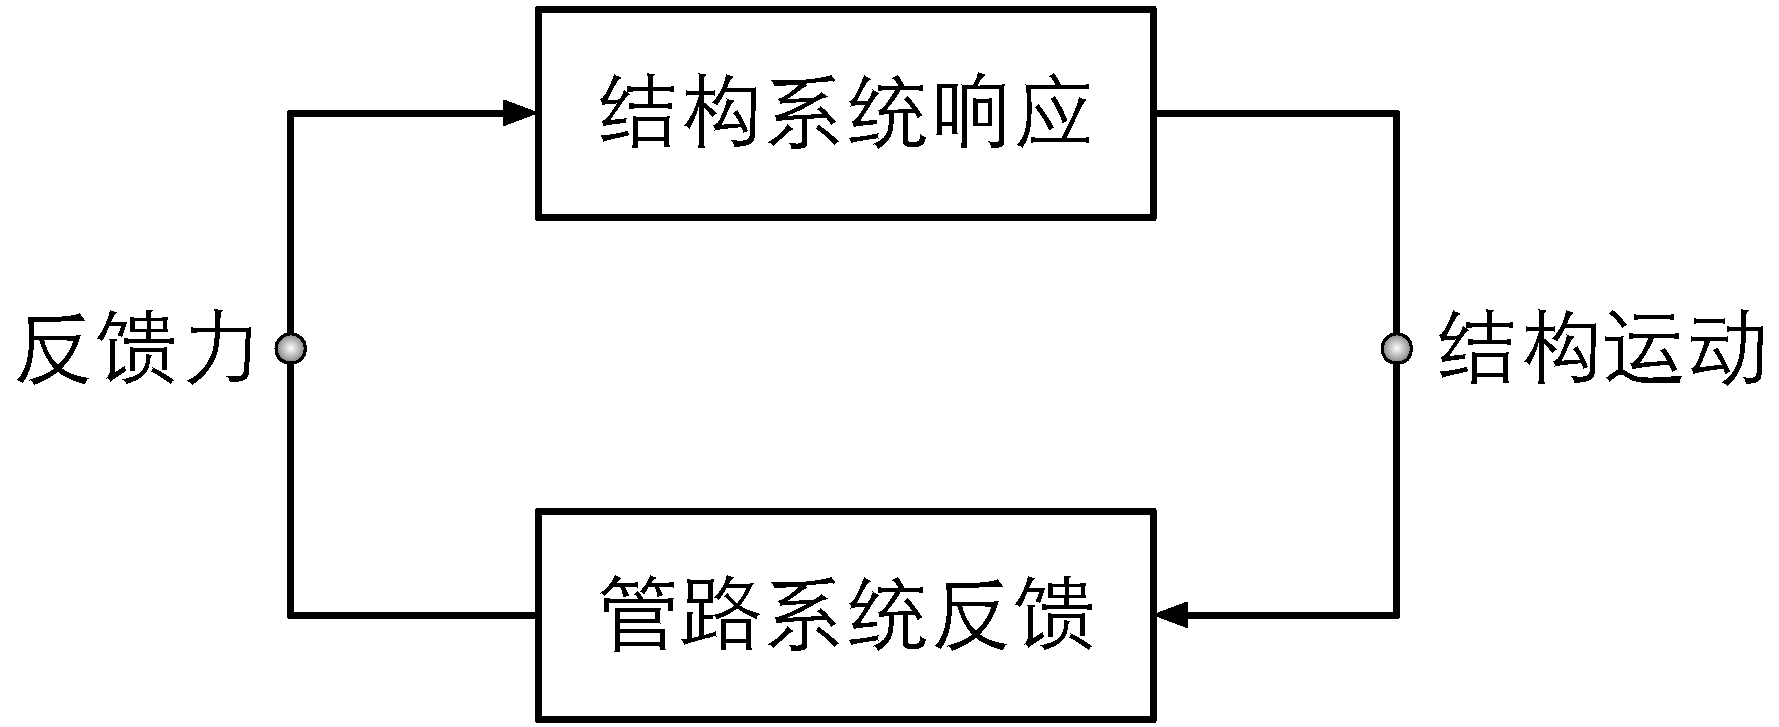
\includegraphics[width=.6\linewidth]{Struture-Feedline-Interaction-Diagram.pdf}
  \caption{POGO振动示意框图}\label{Interaction-Diagram}
\end{figure}

除去一种不常见的增压气体耦合POGO振动\cite{Rubin:1970},典型的POGO闭环振动究其原因可以归纳为如下过程(图\ref{Interaction-Diagram}):在大型液体运载火箭飞行的过程中,燃烧剂和氧化剂输送管路内的液路压力和流量会因为火箭结构系统的扰动而产生脉动。此脉动量经过不同管路元件的层层传递,最终将会到达液体火箭燃烧室,进而引起发动机产生推力脉动。此外,在燃烧剂和氧化剂的输运过程中,管路系统也会由于液体和管壁发生流固耦合作用而产生作用于结构系统上的额外反馈力\cite{About:1987, Paidoussis:1993}。所以当发动机推力脉动,联合上述管路系统反馈力,作为外界扰动力反作用于箭体结构时,火箭结构系统和管路推进系统两者就有可能因为固有频率相接近而产生不断放大耦合作用,从而导致液体推进火箭产生自激的纵向不稳定振动\cite{Rubin:1970, Oppenheim:1993}。

\begin{figure}[!htb]
  \centering
  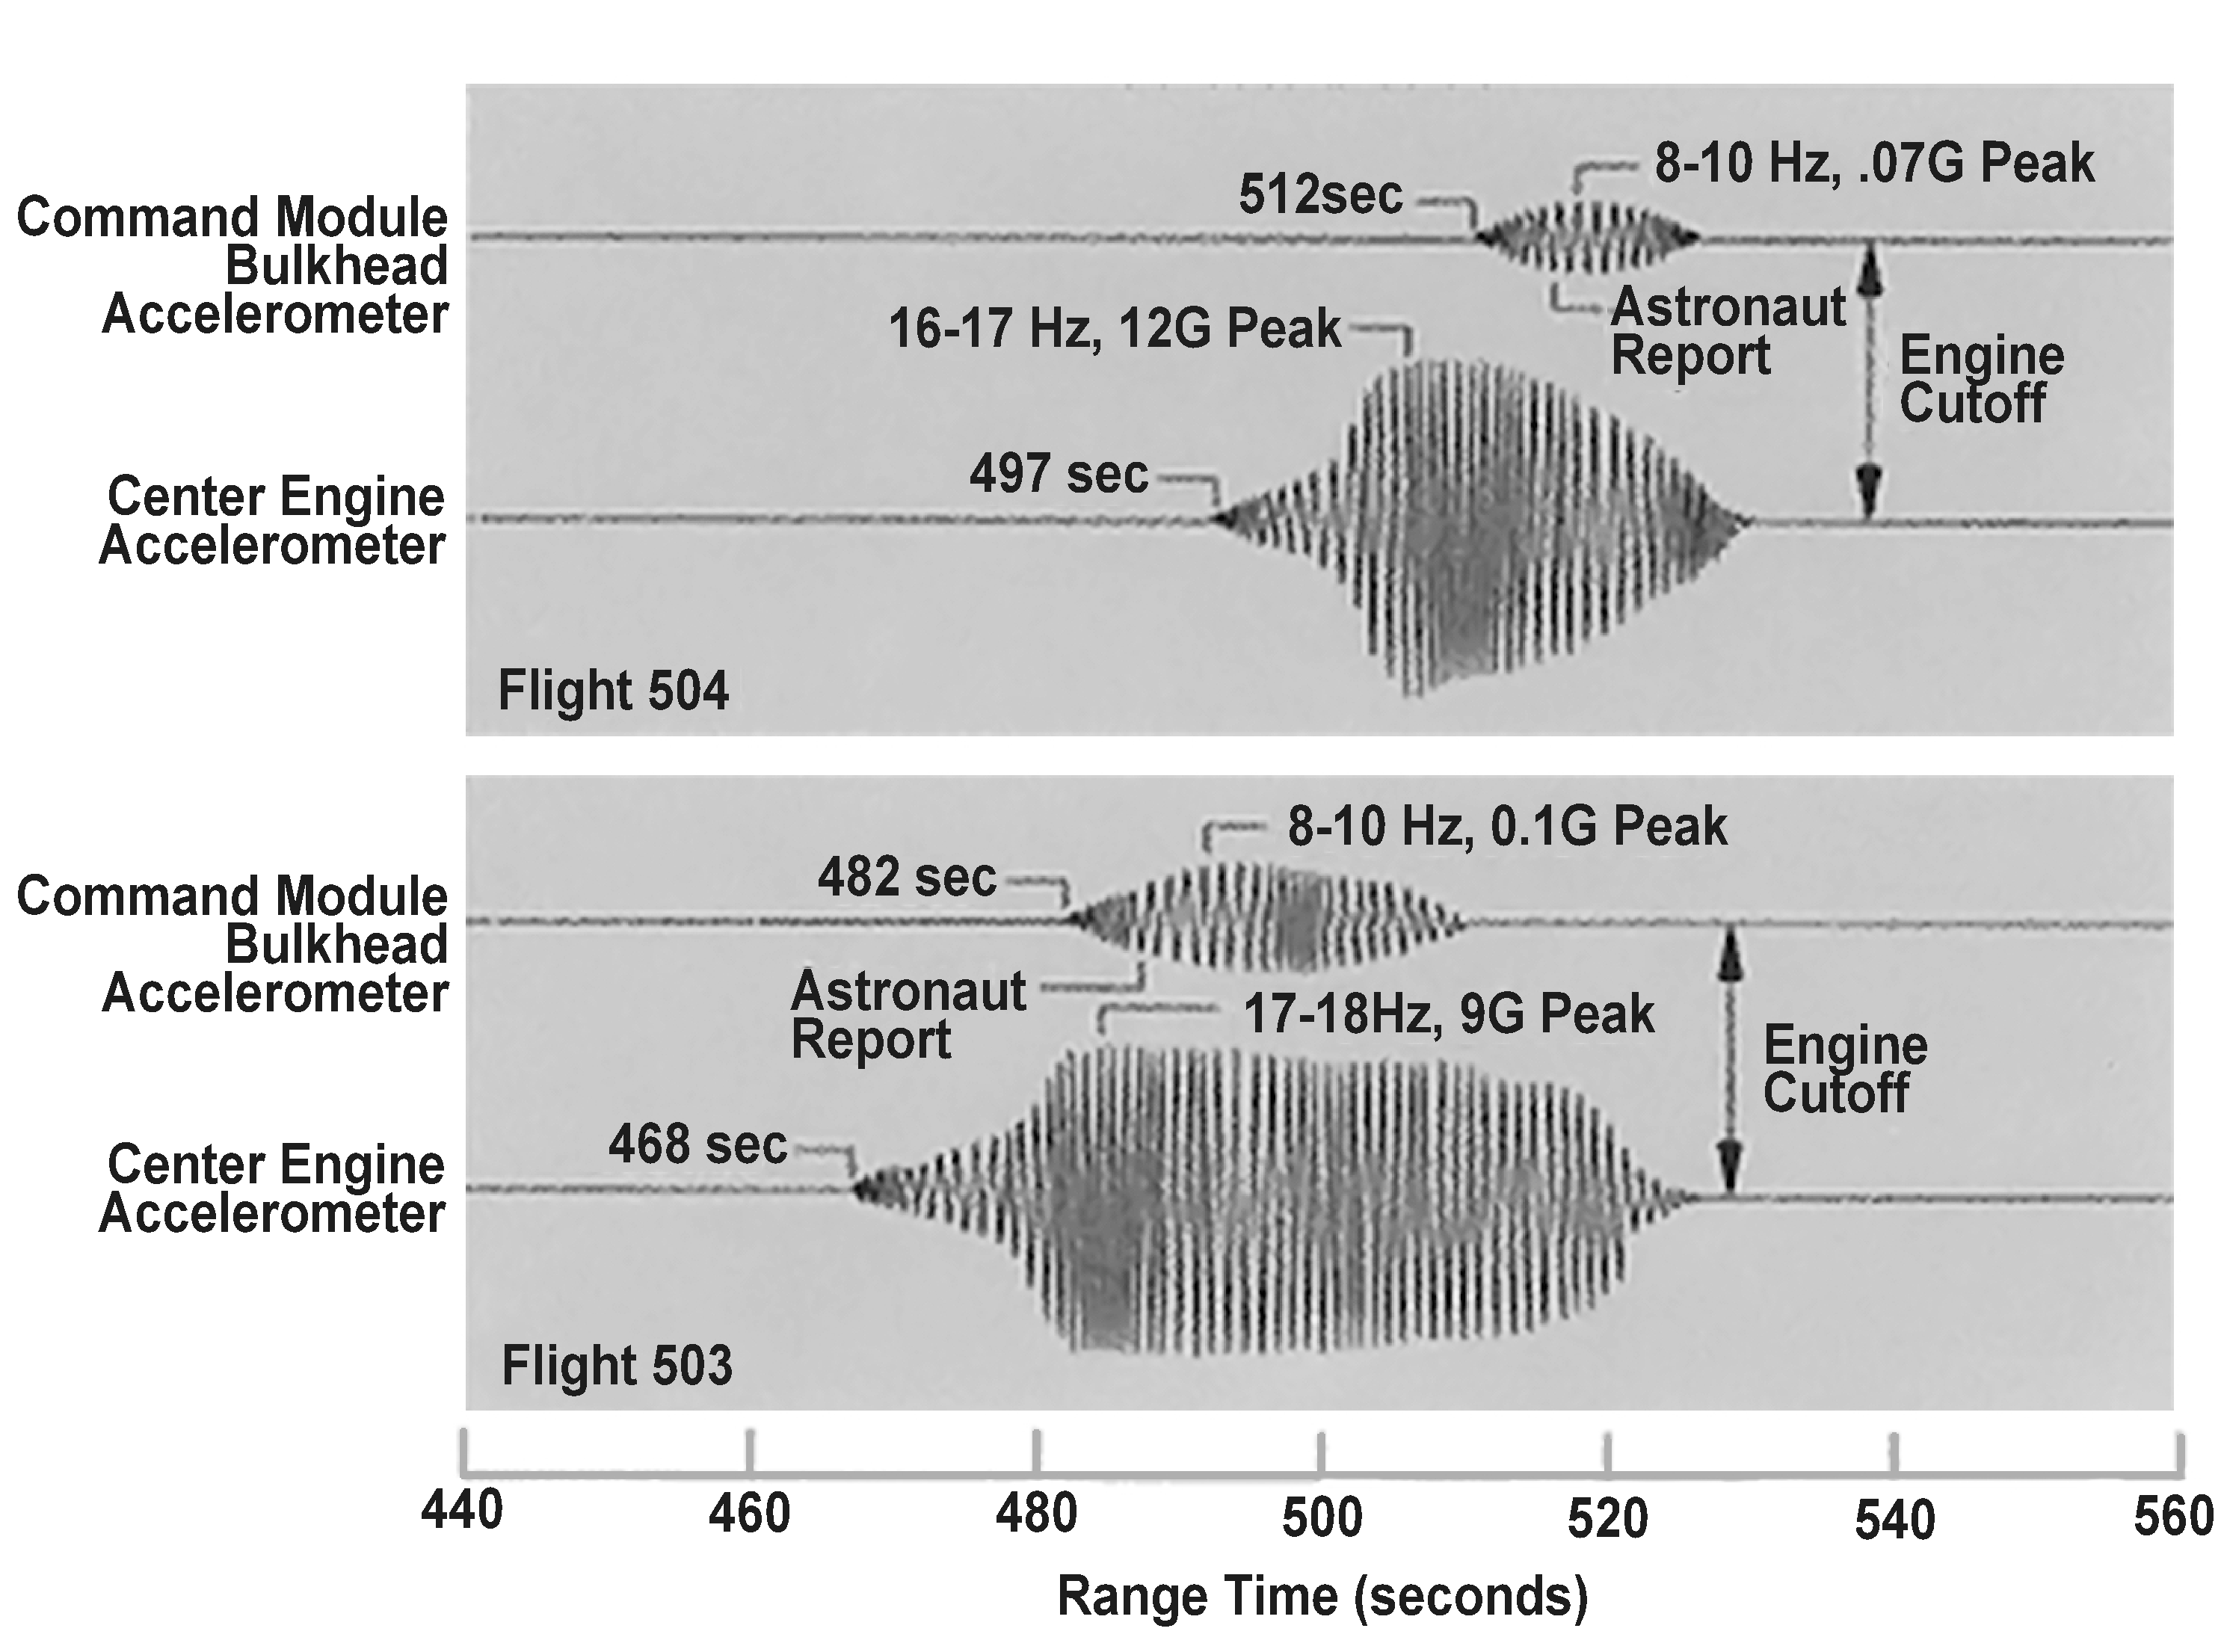
\includegraphics[width=\linewidth]{telemetry-typical.pdf}
  \caption{土星V箭体加速度传感器数据}\label{telemetry-typical}
\end{figure}

参考POGO振动的发生机理并结合国内外大量的飞行遥测数据\cite{Feng-Zhenxing:1981},可以知道这种不稳定振动的发生频率大多与火箭结构系统的低阶纵向振动频率较为接近,其产生和发展过程也表现的十分突然和强烈。事实表明,POGO振动可能发生在液体火箭飞行过程的各个时刻,一次发射也确实可能会出现多次的POGO 振动\cite{Larsen:2008}。然而,由于液体火箭飞行过程是一个持续的变结构参数过程,并且箭体结构在发生较大变形时所引起的非线性效应会打破上面描述的这种频率耦合,所以即使出现POGO 现象,箭体振动的幅值也不会一直发散,而是在其响应时间的历程记录曲线上会出现一个先增大后减小的“鼓包”,典型的遥测POGO振动图像如图\ref{telemetry-typical}所示。鉴于POGO振动从发生到完全消失的时间可能长达数十秒,并且由其引起的箭体纵向振动加速度幅值可能在有效载荷处高达十几甚至几十倍于重力加速度,所以POGO振动对于液体火箭所造成的影响需要根据这种自激振动的量级及持续的时间来进行评价\cite{Wang-Qizheng:1999}。



\section{本文的主要工作}

\begin{figure}[!b]
  \centering
  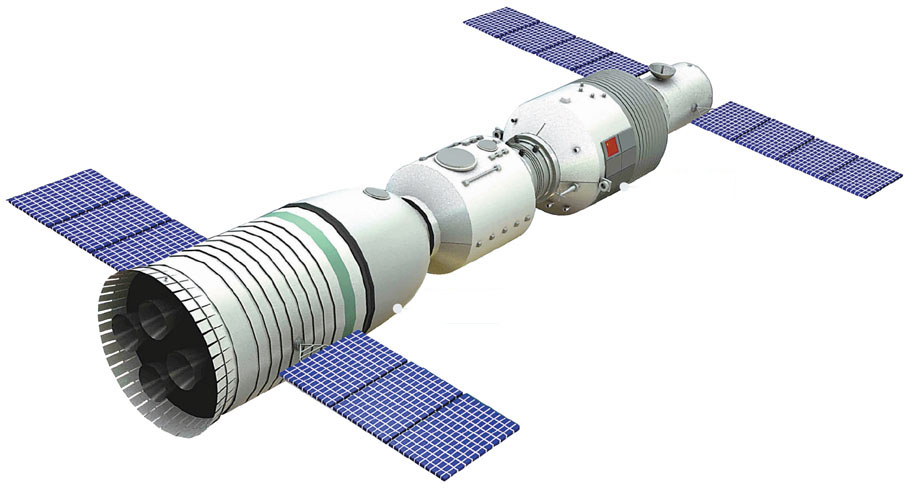
\includegraphics[width=.85\linewidth]{Inter-connect.jpg}
  \caption{神舟十号与天宫一号交汇对接示意图}\label{China-Manned-Flight}
\end{figure}

液体火箭纵向耦合振动问题是一个相对古老却又富含新鲜挑战和契机的复杂系统问题。在我国大力发展航空事业的今天(图\ref{China-Manned-Flight}),更被赋予了深层次的时代意义。传统的液体火箭POGO稳定性分析方法主要分为了矩阵法、单传法和临界阻尼法\cite{Wang-Qizheng:1999}等几类。这些方法都需要先计算出耦合系统的闭环或者开环传递函数,然后通过对系统传递函数进行特征值求解或者绘制Bode和Nyquist图等手段来进行POGO稳定性分析。不过,由于耦合系统的传递函数通常都包含了一些复杂的非线性函数,所以POGO稳定分析的理论难点其实可以被归结为如何快速精确地计算出复杂传递函数的特征值这一经典问题。以矩阵法为例,由于系统反馈力传递矩阵中的元素包含了超越函数和高阶多项式,所以需要对不对称的复数传递矩阵进行非线性复特征值求解,而通常这种非线性方程的求解过程都十分困难并且容易漏根\cite{Dennis:1983, Golub:1996}。正是考虑到此类特征值问题的复杂性,Oppenheim\cite{Oppenheim:1993}等人如前所述,尝试了利用有限元法对管路系统进行直接建模。事实证明,这种方法在处理简单液路元件的组装计算方面确实具有着很高的可操作性和精确度。然而,由于管道内的流体运动问题归根结底是一个复杂的非线性问题\cite{Munson:1990, Paidoussis:1993, Morand:1995},所以当简单流体模型不能够精确描述管路系统传递关系,而研究者们必须要考虑诸如边界层效应,甚至湍流等复杂流体运动的时候,经典的有限元方法就必须被进一步拓展才能适应研究需要,而这种扩展可能相比于直接求解非线性特征值问题更加棘手。除此之外,由于流体单元本构关系的构建严重依赖于液路元件实验参数(如液路惯性,阻抗等)的精确标定,而相比于直接测定各类液路元件的工作参数,标定管路系统的总体反馈力传递函数可能会显得更加方便并且直接。所以,本文在POGO稳定性求解方法的研究方面,直接针对于管路系统的反馈力传递函数展开分析,开辟了另外一种与液路元件有限元组装法平行的POGO振动问题快速特征值求解方法。

为了解决上述主要问题,本文将研究工作分为了以下三个部分:

\begin{enumerate}[label=\textbf{\Roman*.}, align=left, leftmargin=0pt, listparindent=\parindent, itemindent=!, labelwidth=\parindent, labelsep=0pt, itemsep=1em]
\litem{集中参数模型的POGO稳定性分析(第二章)} 本章主要介绍了液体火箭结构系统和管路推进系统典型液路元件的集中参数模型建模方法,发展了一种基于矩阵法和有理分式拟合法的耦合系统快速特征值求解算法。首先推导了各类管路元件上下游脉动压力、流量之间的传递函数关系,结合发动机燃烧室的压力平衡条件与贮箱底部实际边界条件,综合分析出了管路系统反馈于结构系统的力传递函数。接下来,利用快速特征值求解方法,将包含超越函数的管路推进系统反馈力传递函数等效变换为与结构动力学方程一致的形式,通过求解矩阵特征值问题确定了耦合系统的动力学稳定性问题。最后,通过与传统矩阵法进行计算结果和效率方面的比对,验证了该方法的可靠性和高效性。
\litem{基于三维带液贮箱模型的POGO稳定性分析(第三章)} 为了更好的模拟火箭贮箱内液体和结构系统之间的流固耦合效应,引入液体火箭贮箱的三维轴对称模型建模方法,并利用虚质量法对贮箱内的液体进行动力学比拟。发展后的三维带液贮箱模型为管路系统提供了更为科学和精确的入口端边界条件,可以同样利用第二章中描述的管路系统类结构化建模方法,结合MSC.Nastran提供的传递函数TF卡建模工具,将拟合完毕的管路系统传递函数与不同类型的结构系统模型进行耦合计算。通过直接计算耦合系统的复特征值问题,可以方便的得知耦合系统的POGO稳定性。此外,计算过程还考虑了POGO稳定性分析中的另外一项关键性技术,即结构系统阻尼特性的识别和建模。带液贮箱的模态实验表明:在满箱、半箱和空箱等不同状态下,火箭结构系统的阻尼特性存在着较大差异,且半箱状态下结构阻尼较其他状态有明显增大。通过调整贮箱干/湿面材料随时间变化的比例阻尼系数,计算模型成功模拟了上述模态实验结果。最终,通过与实际火箭发射的遥测数据进行对比,证明了本套方法可以快速准确的得出POGO出现时间和振动特性。
\litem{液体火箭POGO稳定性参数分析及传递特性分析(第四章)} 通过比较不同工况下液体火箭POGO稳定性分析结果,本章首先揭示了耦合系统特征值与管路系统关键参数(如蓄压器容积等)之间的相互联系。分析表明,作为POGO抑制器的蓄压器,其容积变化能够显著影响液体火箭管路系统的固有频率,继而改变耦合系统的POGO稳定性。此外,通过比较不同类型液体火箭的历史遥测数据,可以发现有效载荷(如卫星等)的实际振动状态与液体火箭整体POGO振动的强弱并不存在简单的线性关系,单纯的耦合系统特征值计算并不能完全展现液体火箭各处的真实振动状态。文章最后指出,若要使得POGO稳定性分析能够给予未来的发射任务以实质性指导意见,还需综合考虑耦合系统的加速度传递特性分析。
\end{enumerate}